\documentclass[18pt]{beamer}

%%%%%%%%%%%%%%%% Título/Autores %%%%%%%%%%%%%%%%%%%%%%%%
\title[]{
{\fontsize{28pt}{30}\selectfont\textbf{Introdução ao Django}}}
\author{
{\fontsize{18pt}{20}\selectfont \textbf{
Arnaldo Correia, IFBA  arnadocorreia@outlook.com
}}}


%%%%%%%%%%%%%%%% Configurações %%%%%%%%%%%%%%%%%%%%%%%%
%%%%%%%%%%%%%%%% Tema %%%%%%%%%%%%%%%%%%%%%%%%
\mode<presentation> {
\usetheme{Madrid}
\usecolortheme{dove}

}

%%%%%%%%%%%%%%%% Pacotes %%%%%%%%%%%%%%%%%%%%%%%%


\usepackage[brazil]{babel}
\usepackage{color}	
\usepackage[T1]{fontenc}
\usepackage[utf8]{inputenc}	
\usepackage{txfonts}

% To define colors 
\definecolor{ferngreen}{rgb}{0.31, 0.47, 0.26}

% To hide bottom navigation symbols in beamer
\setbeamertemplate{navigation symbols}{}

\usepackage{times}
\usepackage{graphicx,epsfig,psfrag,float,color}
\usepackage{tikz}
\usepackage{pgfplots}
\pgfplotsset{compat=1.15}

\usefonttheme[onlymath]{serif}
\usepackage{amsmath,amssymb,amsfonts,amsthm,mathrsfs}

\usepackage{lmodern} 

\usepackage{scalefnt}
\usepackage{ragged2e} % Justifica o texto no slide
% Testando citação 
\setbeamertemplate{frametitle continuation}[from second]

% Para citações
\usepackage{url}
\usepackage{hyperref}
% ----------

%%%%%%%%%%%%%%%% Logos %%%%%%%%%%%%%%%%%%%%%%%%

% Logo no corpo do texto
\logo{%
  \makebox[0.95\paperwidth]{%
   %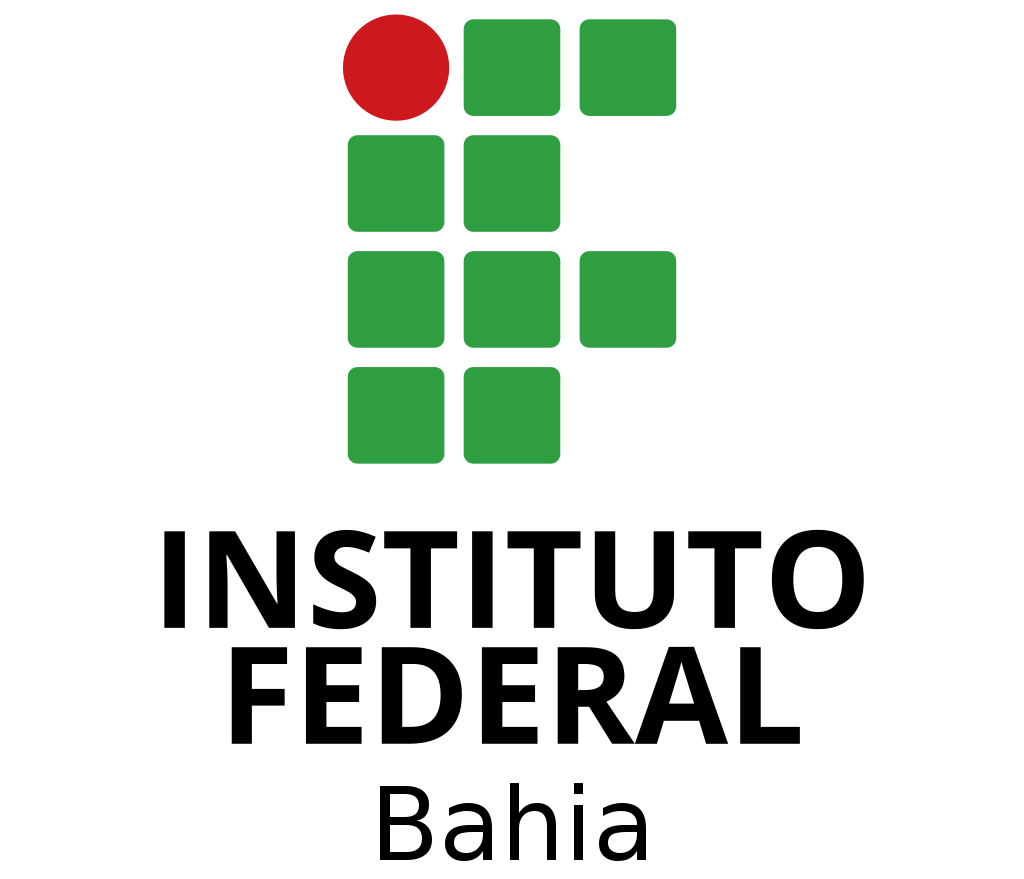
\includegraphics[width=1.6cm,keepaspectratio]{Figures/marca.png}
    \hfill%
    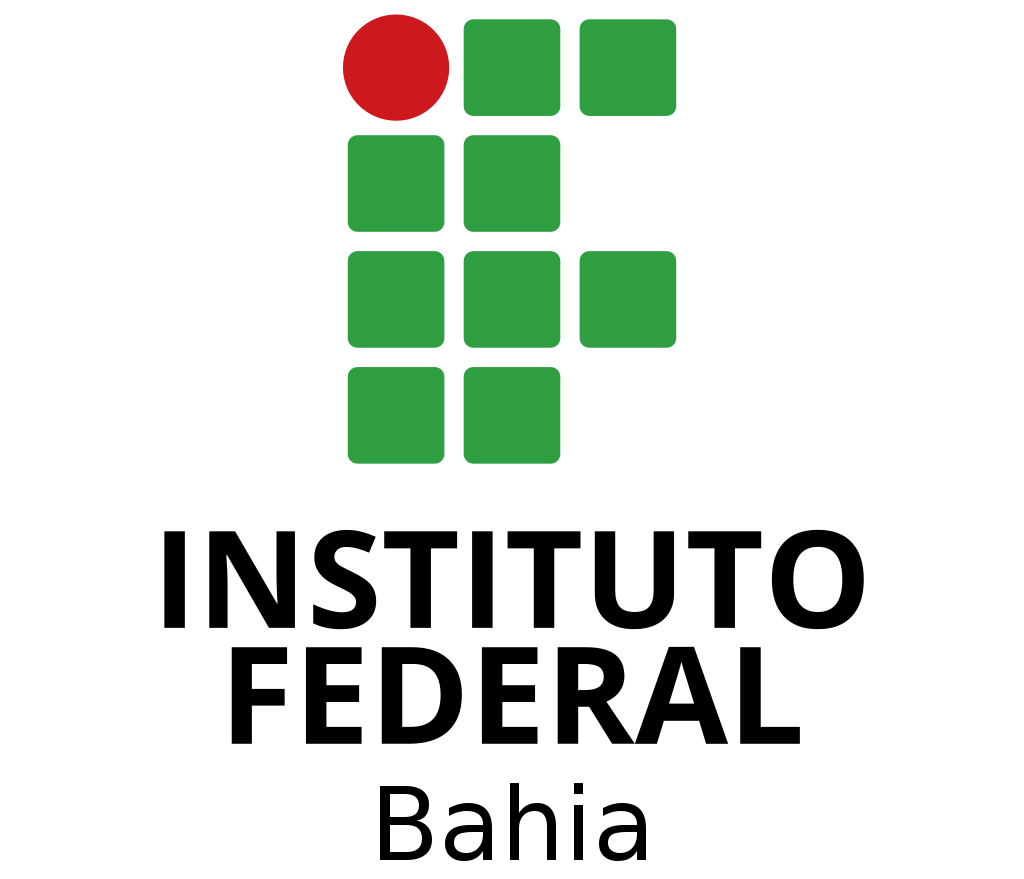
\includegraphics[width=1.3cm,keepaspectratio]{Figures/marca.png}%
  }%
\vspace{200pt}}

%Para inserir o logo no título
\newcommand{\logotitle}{\setbeamertemplate{logo}{
  \makebox[0.95\paperwidth]{%
    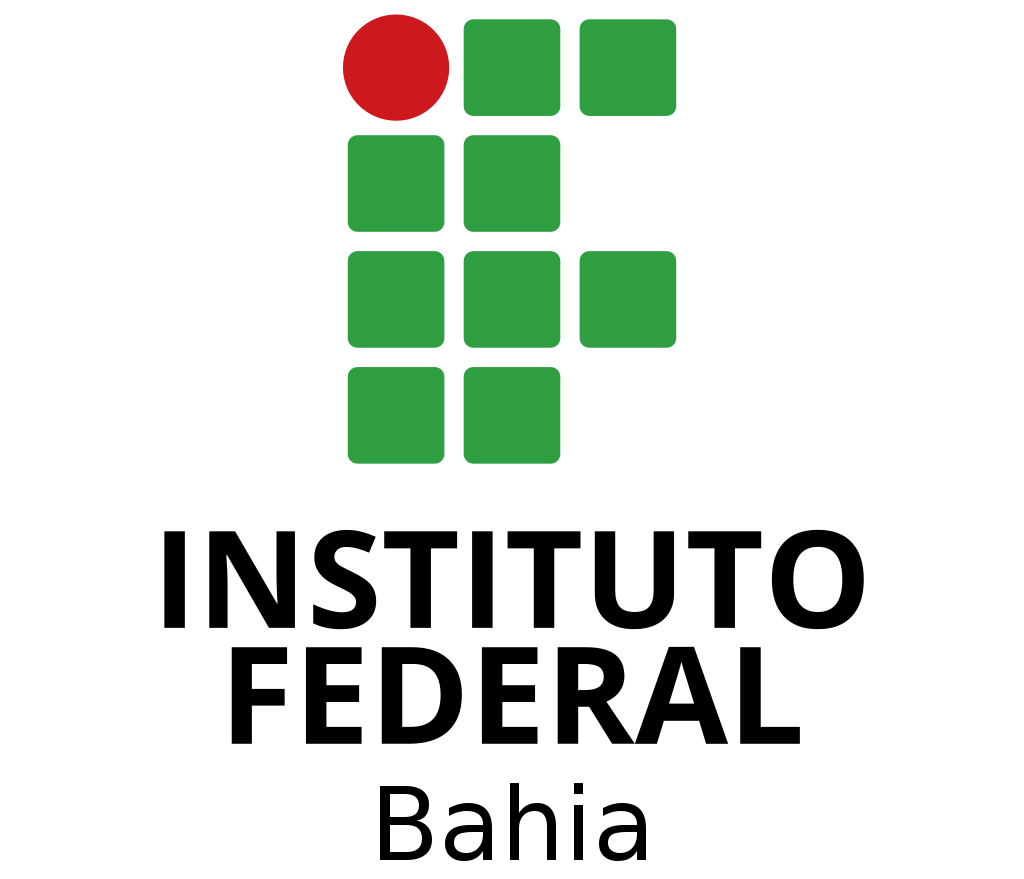
\includegraphics[width=1.3cm,keepaspectratio]{Figures/marca.png}%
    \hfill%
    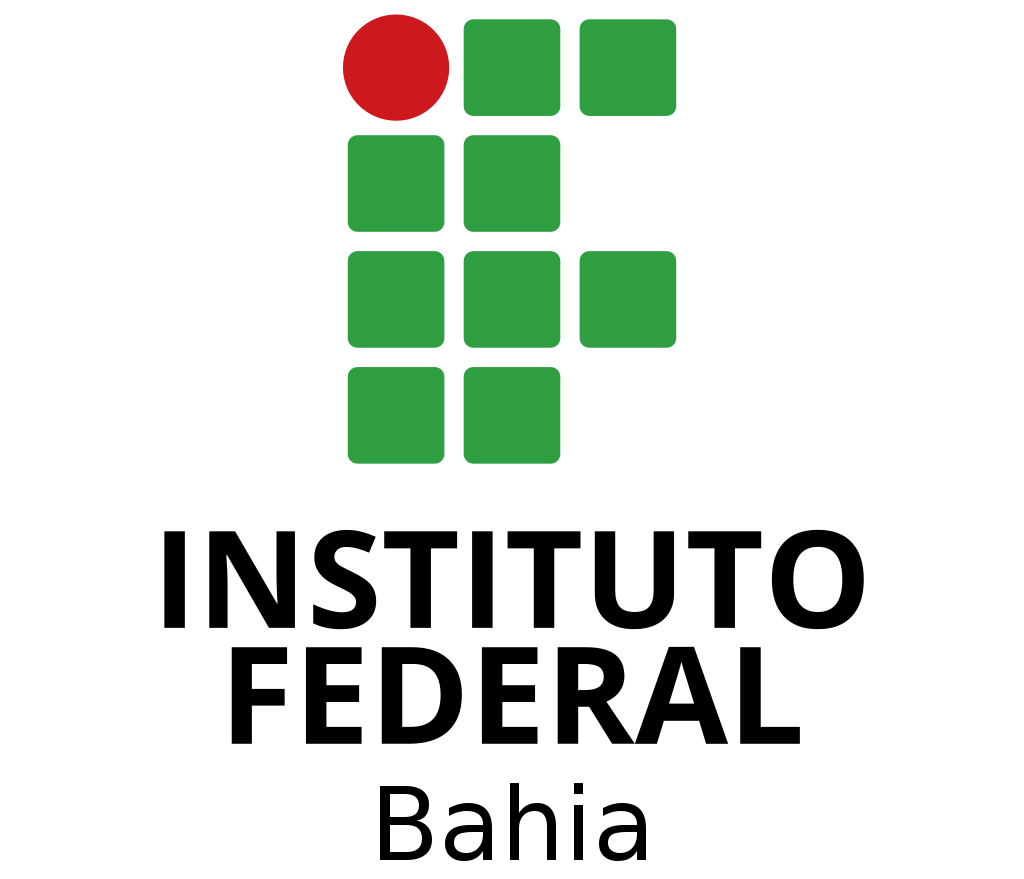
\includegraphics[width=1.3cm,keepaspectratio]{Figures/marca.png}%
  }%
\vspace{220pt}
}}

% To not put logos
\newcommand{\nologo}{\setbeamertemplate{logo}{}}


%%%%%%%%%%%%%% Notas de rodapé %%%%%%%%%%%%%%%%%%%%

\renewcommand{\insertshorttitle}{{\fontsize{8pt}{8}\selectfont { IFBA }}}
\renewcommand{\insertshortauthor}{{\fontsize{8pt}{8}\selectfont {\today }}}
\date{}
 

\setbeamertemplate{footline}{
   \begin{beamercolorbox}[ht=2ex,leftskip=2mm,rightskip=2mm]{}
   % ht: altura
    \textcolor{ferngreen}{\hrule height 5pt}
    \vspace{0.3cm}
    \insertshortauthor \hfill \insertshorttitle  \hfill  {\fontsize{8pt}{8}\selectfont {\insertframenumber}}
   \end{beamercolorbox}
   \vspace*{0.3cm}
} 




\begin{document}

%------------------------------------------------------
{\logotitle
\begin{frame}
\maketitle
\end{frame}
}

%------------------------------------------------------


\begin{frame}{\fontsize{20pt}{20}\selectfont \textbf{Introdução}}

  Django é um framework de aplicativos web gratuito e de código aberto escrito em python
  que segue o padrão arquitetural MVC (Model View Controller).
  \newline
  Model -> É o responsável por fazer a comunicação com os bancos de dados.
  \newline
  View -> É onde os dados são visualizados.Podemos incluisive ter várias visões HTML,TEXTO.
  \newline
  Controller -> É onde as views e os modelos se comunicam.

\end{frame}


%------------------------------------------------------

\begin{frame}{\fontsize{20pt}{20}\selectfont \textbf{Objetivo(s)}}



\end{frame}


%------------------------------------------------------
\begin{frame}{\fontsize{20pt}{20}\selectfont \textbf{Metodologia}}



\end{frame}


%------------------------------------------------------
\begin{frame}{\fontsize{20pt}{20}\selectfont \textbf{Resultados}}

\begin{itemize}
    \item Resumos expandidos
    \begin{itemize}
        \item Devem apresentar resultados esperados ou obtidos se for o caso;
    \end{itemize}
    \item Artigos completos
    \begin{itemize}
        \item Devem apresentar resultados obtidos.
    \end{itemize}
\end{itemize}

\end{frame}


%------------------------------------------------------
\begin{frame}{\fontsize{20pt}{20}\selectfont \textbf{Conclusões e trabalhos futuros}}



\end{frame}


%------------------------------------------------------
\begin{frame}[allowframebreaks] {\fontsize{20pt}{20}\selectfont \textbf{Normas para apresentação de trabalhos}}

\begin{itemize}
{\fontsize{11pt}{11}\selectfont
    \item Este documento apresenta a estrutura base da apresentação oral;
    \item O trabalho deverá ser apresentado obrigatoriamente por um dos autores;
    \item O autor terá até 10 minutos para apresentação oral;
    \item O apresentador deverá comparecer com pelo menos 20 minutos de antecedência na sala de sua apresentação;
    \item Após a apresentação haverá 5 minutos para que o autor possa responder perguntas ou esclarecer dúvidas dos participantes;
    
    \framebreak
        
    \item Em todas as salas será disponibilizado data-show e computador para apresentação;
    \item Cada sala terá, no mínimo, um chair da seção;
    \item O certificado de apresentação de trabalho será enviado até 60 dias do término do congresso por e-mail;
    \item A sequência e os horários de apresentação dos trabalhos foi disponibilizada no site do congresso;
    \item Caso o trabalho não seja apresentado, não será emitido certificado e não constará  nos anais do evento.}
\end{itemize}

\end{frame}

%%%%%%%%% References %%%%%%%%
\nocite{*}
\begin{frame}[allowframebreaks] 
\frametitle{\fontsize{20pt}{20}\selectfont \textbf{Referências}}
{\scriptsize
\bibliographystyle{apalike}
\bibliography{References.bib}
}
\end{frame}



%------------------------------------------------------

\end{document}
